\section{Validierung}
Im folgenden Abschnitt wird die Validierung beschrieben. Die Validierung dient zum Auffinden und Beheben von Fehlern, um so eine korrekte Funktion des Programms garantieren zu k�nnen. Zum einen wurden die Berechnungen und Simulationen von Matlab �berpr�ft, zum anderen die Software, aufgeteilt in die Teilbereiche Benutzeroberfl�che und Berechnungen.

\subsection{Matlab}

\subsubsection{Programmierung}
%Problem/Fragestellung:
%- Wie kann die korrekte Funktion der Matlab-Programme �berpr�ft werden?
%L�sung: Die berechneten Antworten werden mit den Antworten von Herrn Niklaus verglichen.
Die Berechnung der Regler wurde zuerst mittels m-Files in Matlab implementiert. Zur �berpr�fung der von Matlab gelieferten Werte wurden diese mit den Werten vom Fachcoach Peter Niklaus verglichen.


\subsubsection{Simulation}
%Problem/Fragestellung:
%- Wie kann die Matlab-Simulation �berpr�ft werden?
%L�sung: Sie wird mit Simulink �berpr�ft.
Mittels Simulink wurde der geschlossene Regelkreis simuliert.

\subsection{Java Software}

\subsubsection{Benutzeroberfl�che}
%Problem/Fragestellung:
%- Wie k�nnen Probleme oder Konflikte bei der Benutzeroberfl�che ausgeschlossen werden?
%Mehrere unabh�ngige User testen die Software.

%Um die einfache Handhabung der Software zu �berpr�fen wurde die Software im ganzen Projektteam sowie von mehreren unabh�ngigen Benutzern getestet. Die so gefundenen Unklarheiten oder Probleme wurden behoben.

\subsubsection{Model}
%Problem/Fragestellung:
%- Wie wird die korrekte Funktion der Software �berpr�ft?
%L�sung: Die Software mit mit JUnit getestet, wobei die Resultate von Matlab erwartet werden.
Die Plausibilit�t der Schrittantworten konnte relativ einfach optisch mit den Graphen �berpr�ft werden, da das Verhalten der einzelnen Regler bekannt ist. Zur genauen �berpr�fung der einzelnen Klassen wurden s�mtliche Klassen des Models mittels JUnit mit den Ergebnissen von Matlab verglichen.

\subsubsection{Performancevergleich Partialbruchzerlegung und IFFT}\label{residuenvsifft}
Es wurde festgestellt dass das Berechnen des Schrittantwortes mittels IFFT-Methode merkbar langsam ist - vorallem dann, als das iterative Approximieren des �berschwingens implementiert wurde, was dazu f�hrte, dass die Schrittantwortberechnung mehrmals ausgef�hrt werden musste.

Durch Reduzieren der Anzahl Pünkte kann die Berechnung beschleunigt werden, jedoch kommt dies auf Kosten von Genauigkeit.

\begin{figure}
\centering
\begin{subfigure}{.33\textwidth}
	\centering
	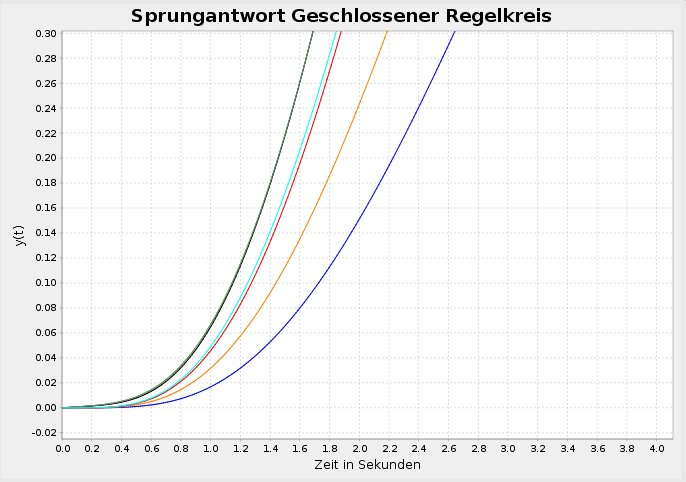
\includegraphics[width=.2\linewidth]{./ifft_4096.jpg}
	\caption{A subfigure}
	\label{fig:sub1}
\end{subfigure}
\begin{subfigure}{.33\textwidth}
	\centering
	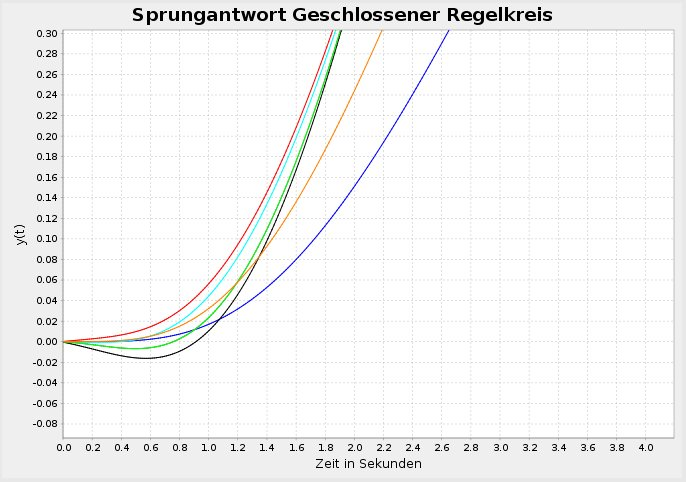
\includegraphics[width=.2\linewidth]{./ifft_2048.jpg}
	\caption{A subfigure}
	\label{fig:sub2}
\end{subfigure}
\begin{subfigure}{.33\textwidth}
	\centering
	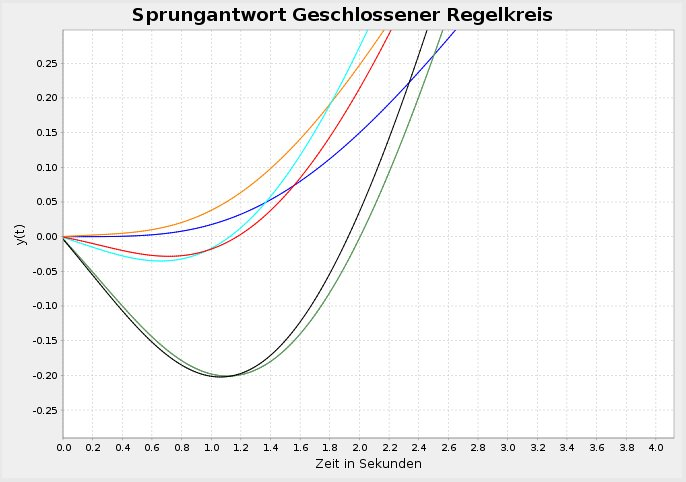
\includegraphics[width=.2\linewidth]{./ifft_1024.jpg}
	\caption{A subfigure}
    \label{fig:sub3}
\end{subfigure}
\caption{A figure with three subfigures}
\label{fig:test}
\end{figure}

Es wurde entschieden, eine alternative Berechnungsmethode zu implementieren: Schrittantwortberechnung mittels Partialbruchzerlegung.

